%\documentclass[aps, twocolumn]{revtex4}
\documentclass[aps]{revtex4}
\usepackage{graphicx}
\DeclareGraphicsExtensions{.pdf,.eps}

%\pagestyle{empty}


%% Macros:

\newcommand{\srr}[1]{\stackrel{\rightharpoonup\!\!\!\!\rightharpoonup }{#1}}
\newcommand{\Tep}[0]{\srr{\cal\varepsilon}}
\newcommand{\Tepmain}[0]{\Tep_{\!\!main}}
\newcommand{\Tup}[0]{\srr\Upsilon}
\newcommand{\Ttau}[0]{\srr{\cal\tau}}
\newcommand{\Tpi}[0]{\srr{\cal\pi}}
\newcommand{\TI}[0]{\srr I}
\newcommand{\mbf}[0]{\mathbf f}
\newcommand{\mbF}[0]{\mathbf F}
\newcommand{\bh}[0]{\mathbf h}
\newcommand{\br}[0]{\mathbf r}
\newcommand{\sh}[0]{\mathbf\sigma_{\bh}}
\newcommand{\bT}[0]{\mathbf T}
\newcommand{\bF}[0]{\mathbf F}
\newcommand{\bef}[0]{\mathbf f}
\newcommand{\ba}{\mathbf a}
\newcommand{\bb}{\mathbf b}
\newcommand{\bc}{\mathbf c}
\newcommand{\bhz}[0]{\mathbf h_{0}}
%\newcommand{\bhz}[0]{\mathbf h_{\mathbf 0}}

%\documentstyle[aps,preprint]{revtex}
%%%%%%%%%%%%%%%%%%%%%%%%%%%%
\addtolength{\topmargin}{0.0in}

%% Dimensions:

%% CT> to get holes at left without touching text, changed 
%%       a. margins from -3.5pc to -2pc
%%       b. textheight from 23cm to 24cm
%% CT> 28 SEP 00: makes no sense to use these margins for the version
%%                to be posted on CTAN. Dimens now revert to original
%%                value of  -3.5pc for left/rightmargins. The 
%%                textheight, however, will remain at 24cm.
%%
\setlength{\textwidth}{19cm}
\setlength{\textheight}{24cm}
\setlength{\oddsidemargin}{-3.5pc}
\setlength{\evensidemargin}{-3.5pc}
\setlength{\headsep}{12pt}
\setlength{\topmargin}{-3.5pc}
\setlength{\columnsep}{1.5pc}

%% Fonts:

\font\bfsl=cmssi17
\font\sectiontt=cmtt12 scaled\magstep1
\font\stt=cmtt10 scaled 850





\begin{document}
\title{Routines for the dynamical equations of the period vectors of a crystal under constant external stress}
\author{Gang Liu}
\address{\\
{ e-mail: gang.liu@queensu.ca}\\
{ High Performance Computing Virtual Laboratory}\\
{ Queen's University, Kingston, Ontario, Canada}\\
}

\date{September 04, 2015}


\maketitle

%\newpage






The purpose of this file is to present source code routines for computing the acceleration of the period vectors of a crystal based on the following dynamical equation
\begin{equation}
\alpha _{\bh,\bh} \ddot\bh = \left( \Tpi +\Tup\right ) \cdot \sh\ \ (\bh=\ba, \bb, \bc), \nonumber
\end{equation}
which is the last one before the "SUMMARY AND DISCUSSION" section in our paper \cite{glcjp,glarxiv}.

\section{The FORTRAN 90 Version}

Here is the module of the interface 

\begin{verbatim}
    MODULE PERIOD_ACCELERATION_MDL
       INTERFACE
         SUBROUTINE ACCELERATION_OF_PERIODS( ALPHAS, &
                                    CURRENT_PERIODS, &
                                    INTERNAL_STRESS, &
                                    EXTERNAL_STRESS, &
                               PERIOD_ACCELERATIONS   )
             IMPLICIT NONE
             REAL*8, INTENT(IN) :: ALPHAS(3),            &
                                   CURRENT_PERIODS(3,3), &
                                   INTERNAL_STRESS(3,3), &
                                   EXTERNAL_STRESS(3,3)
             REAL*8, INTENT(OUT):: PERIOD_ACCELERATIONS(3,3)
         END SUBROUTINE ACCELERATION_OF_PERIODS
       END INTERFACE
    END MODULE PERIOD_ACCELERATION_MDL
\end{verbatim} 
where the meaning of each argument is stated by its name. 

However better to further emphasis on those in elementary level.  

The three elements of the \verb!ALPHA! array are the $\alpha _{\bh,\bh}$s for the period vector $\bh=\ba$, $\bb$, $\bc$ in sequence.

The sub-arrays \verb!CURRENT_PERIODS(1:3,1)!,  \verb!CURRENT_PERIODS(1:3,2)!, and  \verb!CURRENT_PERIODS(1:3,3)! 
are the period vectors $\ba$, $\bb$, and $\bc$ respectively. 

The internal stress \verb!INTERNAL_STRESS! array should be 
calculated as the summation of two terms. One is 
the kinetic energy term, which is a scalar as in equation (34) of reference \cite{glarxiv}. The other is the full interaction dyad, which can be 
expressed as
\begin{equation}
\Tep=-\frac 1\Omega \sum_{\mathbf z\in\text{DOF}} \left( \frac{\partial E_{p,MD}}{\partial\mathbf z}\right)\mathbf z,
\label{verynew}
\end{equation}
the last equation of our paper\cite{glcjp,glarxiv}. Be sure here $\mathbf z$ is a vector, not a scalar in the $z$-axis of a usual 
Cartesian coordinate system. For example, the element \verb!INTERNAL_STRESS(1,2)! should contain the element of the above 
equation for  $x$-component of $ \frac{\partial E_{p,MD}}{\partial\mathbf z}$ and  $y$-component of $\mathbf z$. 

\newpage







  \vspace{0cm}
\begin{figure}
  \begin{center}
    \hspace{0cm}
    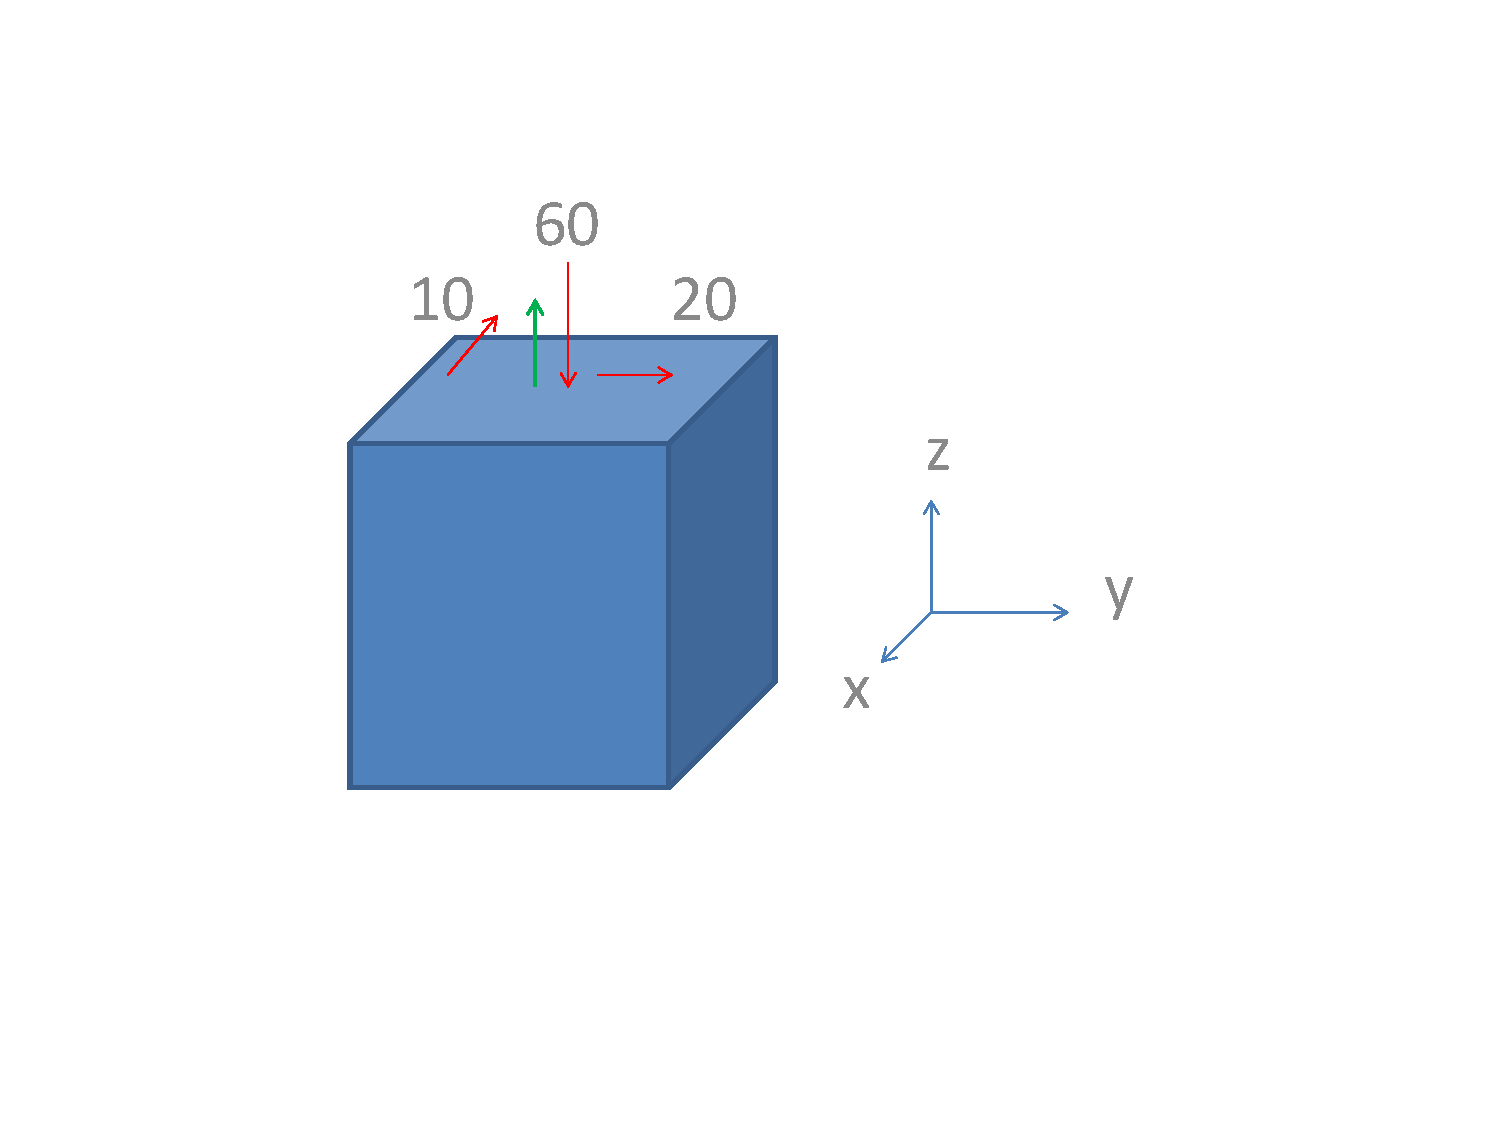
\includegraphics[width=0.7\textwidth]{./anexternalstressexample2.pdf}
  \end{center}
  \vspace{-3cm}
  \caption{External stress on top surface of a crystal. The green arrow is the surface direction. The red arrows are the directions of the external forces and the numbers are the corresponding absolute values per unit area.}
  \label{fig1}
\end{figure}

  \vspace{2cm}
The external stress \verb!EXTERNAL_STRESS! array is straight-forward. However much attention should be paid to the (positive or negative) sign of each element. For the (red) external forces per unit area acting on the top surface of a crystal as illustrated in Fig. 1, the \verb!EXTERNAL_STRESS! should be set as (with symmetry property considered)
  $ \left( \begin{array}{rrr}
           u &   v &    -10 \\ 
           v &  w &  20 \\ 
           -10 &  20 &   -60
            \end{array}
     \right)  
  $,
where $u$, $v$, and $w$ should be based on the external forces applied on the side surfaces. When this external stress is applied on the bottom surface of the crystal in Fig. 1, the forces are of the same amplitude but in the opposite directions compared with those on the top surface. When the crystal reaches an equilibrium state, the internal stress must be
  $ \left( \begin{array}{rrr}
           -u &  - v &    10 \\ 
           -v &  -w &  -20 \\ 
           10 &  -20 &  60
            \end{array}
     \right)  
  $.




The  \verb! PERIOD_ACCELERATIONS(1:3,1)!,  \verb! PERIOD_ACCELERATIONS(1:3,2)!, 
and  \verb! PERIOD_ACCELERATIONS(1:3,3)! sub-arrays 
are the accelerations of the period vectors $\ba$, $\bb$, and $\bc$ to be returned respectively. That is the purpose of the routine.



  \vspace{0cm}
The full routine is as follows (next page):

\newpage

\begin{verbatim}
         SUBROUTINE ACCELERATION_OF_PERIODS( ALPHAS, &
                                    CURRENT_PERIODS, &
                                    INTERNAL_STRESS, &
                                    EXTERNAL_STRESS, &
                               PERIOD_ACCELERATIONS   )
             IMPLICIT NONE
             REAL*8, INTENT(IN) :: ALPHAS(3),            &
                                   CURRENT_PERIODS(3,3), &
                                   INTERNAL_STRESS(3,3), &
                                   EXTERNAL_STRESS(3,3)
             REAL*8, INTENT(OUT):: PERIOD_ACCELERATIONS(3,3)
             REAL*8             :: CELL_SURFACES(3,3)
             REAL*8             :: CELL_VOLUME
             INTEGER            :: I, J, K, L, M, N

             DO I = 1, 3
                J = MOD(I, 3) + 1
                K = MOD(J, 3) + 1
                DO L = 1, 3
                   M = MOD(L, 3) + 1
                   N = MOD(M, 3) + 1
                   CELL_SURFACES(L,I) =                              &
                         CURRENT_PERIODS(M,J) * CURRENT_PERIODS(N,K) &
                       - CURRENT_PERIODS(N,J) * CURRENT_PERIODS(M,K)
                END DO
             END DO

             CELL_VOLUME = CELL_SURFACES(1,1) * CURRENT_PERIODS(1,1) &
                         + CELL_SURFACES(2,1) * CURRENT_PERIODS(2,1) &
                         + CELL_SURFACES(3,1) * CURRENT_PERIODS(3,1)

             IF(CELL_VOLUME <= 1.0D-10) THEN
                PRINT*, "Sorry, too small or negative cell volume:"
                PRINT*, CELL_VOLUME
                STOP
             END IF

             DO I = 1, 3
                DO J = 1, 3
                   PERIOD_ACCELERATIONS(J, I) = 0.0D0
                   DO K = 1, 3
                      PERIOD_ACCELERATIONS(J, I) = PERIOD_ACCELERATIONS(J, I) + &
                              (INTERNAL_STRESS(J, K) + EXTERNAL_STRESS(J, K)) * &
                                                          CELL_SURFACES(K, I)
                   END DO
                   PERIOD_ACCELERATIONS(J, I) = PERIOD_ACCELERATIONS(J, I) &
                                              / ALPHAS(I)
                END DO
             END DO

             RETURN
         END SUBROUTINE ACCELERATION_OF_PERIODS
\end{verbatim}


\newpage












\section{The C/C++ Version}

The interface for C/C++ version is
\begin{verbatim}
        void Acceleration_of_PERIODS( double * alphas,
                                      double * current_periods,
                                      double * internal_stress,
                                      double * external_stress,
                                      double * period_accelerations  )
\end{verbatim} 
where the meaning of each argument is stated by its name. All these pointers point to double (one-dimentional) arrays. The first should have at least three elements and all the rest have at least nine elements.

The meaning in elementary level is as follows.  

The three elements of the \verb!alphas! array are the $\alpha _{\bh,\bh}$s for the period vector $\bh=\ba$, $\bb$, $\bc$ in sequence.

The sub-arrays \verb!current_periods[0:2]!,  \verb!current_periods[3:5]!, and  \verb!current_periods[6:8]! 
are the period vectors $\ba$, $\bb$, and $\bc$ respectively, where \verb!an_array[i:j]! means a range of elements from \verb!an_array[i]! to \verb!an_array[j]! 
throughout this document. 

The internal stress \verb! internal_stress! array should be 
calculated as the summation of two terms. One is 
the kinetic energy term, which is a scalar as in equation (34) of reference \cite{glarxiv}. The other is the full interaction dyad, which can be 
expressed as
\begin{equation}
\Tep=-\frac 1\Omega \sum_{\mathbf z\in\text{DOF}} \left( \frac{\partial E_{p,MD}}{\partial\mathbf z}\right)\mathbf z,
\label{verynew}
\end{equation}
the last equation of our paper\cite{glcjp,glarxiv}. Be sure here $\mathbf z$ is a vector, not a scalar in the $z$-axis of a usual 
Cartesian coordinate system. For example, the element \verb! internal_stress[1]! should  contain the element of the above 
equation for  $x$-component of $ \frac{\partial E_{p,MD}}{\partial\mathbf z}$ and  $y$-component of $\mathbf z$. 





\newpage


  \vspace{0cm}
\begin{figure}
  \begin{center}
    \hspace{0cm}
    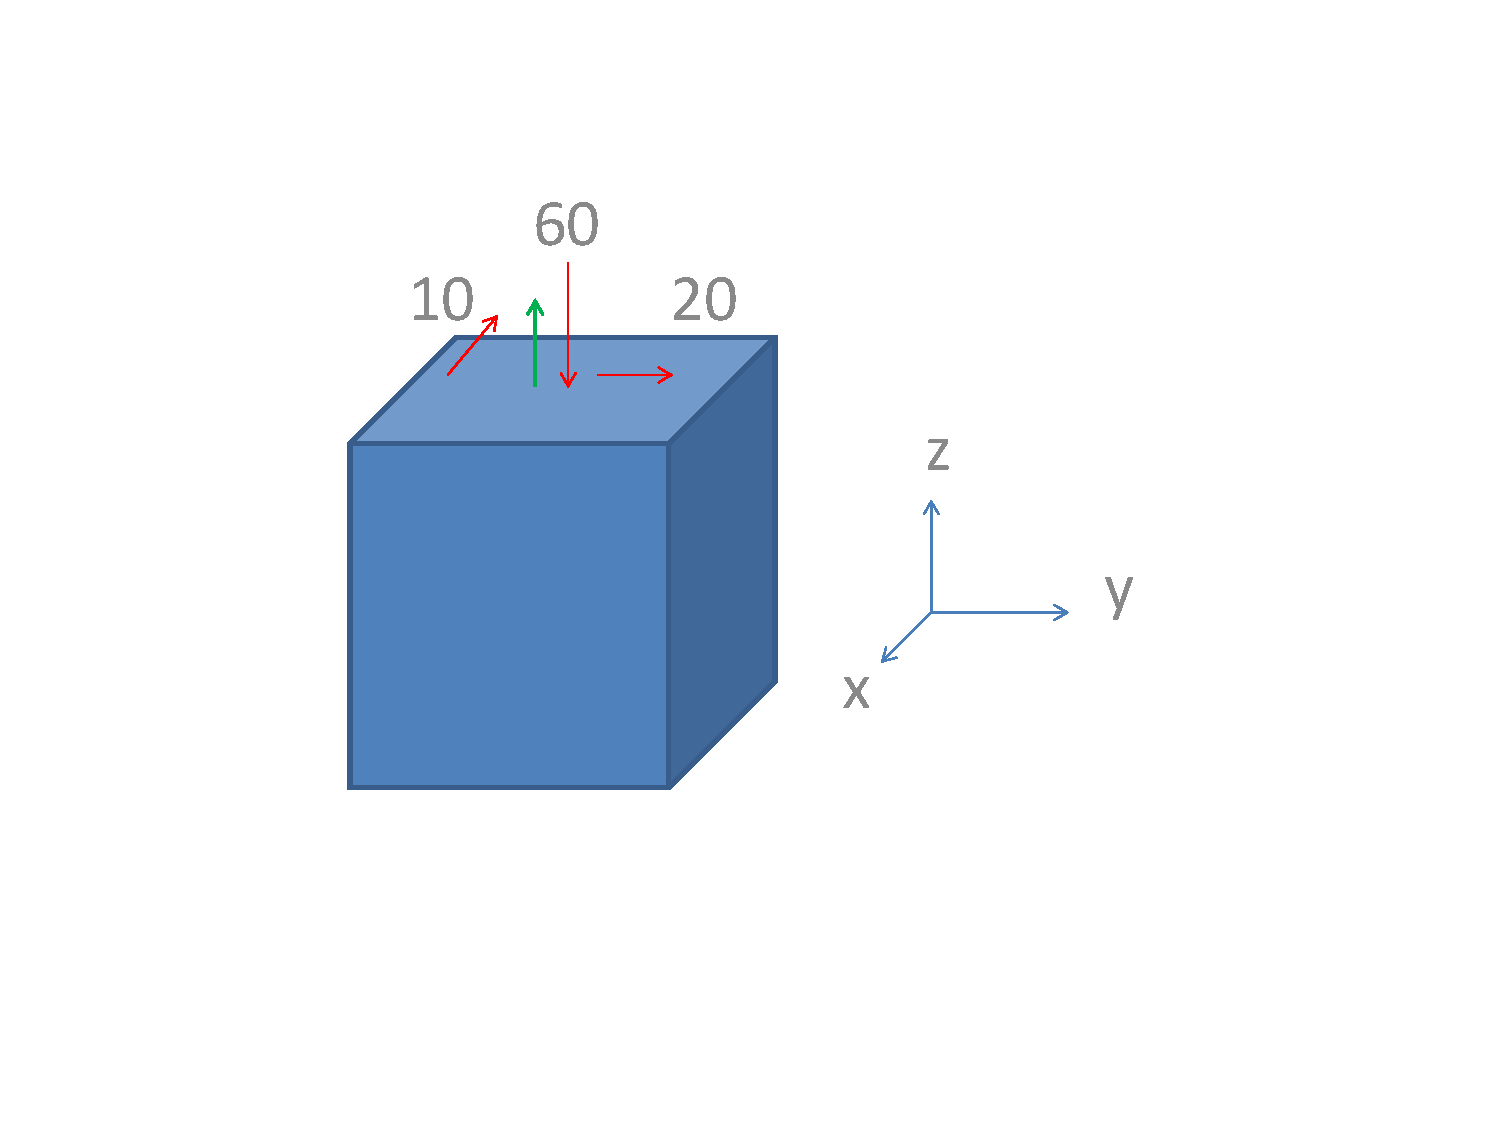
\includegraphics[width=0.7\textwidth]{./anexternalstressexample2.pdf}
  \end{center}
  \vspace{-3cm}
  \caption{External stress on top surface of a crystal. The green arrow is the surface direction. The red arrows are the directions of the external forces and the numbers are the corresponding absolute values per unit area.}
  \label{fig2}
\end{figure}

  \vspace{2cm}
The external stress \verb!external_stress! array is straight-forward. However much attention should be paid to the (positive or negative) sign of each element. For the (red) external forces per unit area acting on the top surface of a crystal as illustrated in Fig. 2, the \verb!external_stress[0-8]! should be set as (with symmetry property considered)
  $ \left( \begin{array}{rrr}
           u &   v &    -10 \\ 
           v &  w &  20 \\ 
           -10 &  20 &   -60
            \end{array}
     \right)  
  $,
where $u$, $v$, and $w$ should be based on the external forces applied on the side surfaces. When this external stress is applied on the bottom surface of the crystal in Fig. 2, the forces are of the same amplitude but in the opposite directions compared with those on the top surface. When the crystal reaches an equilibrium state, the internal stress must be
  $ \left( \begin{array}{rrr}
           -u &  - v &    10 \\ 
           -v &  -w &  -20 \\ 
           10 &  -20 &  60
            \end{array}
     \right)  
  $.




The  \verb!period_accelerations[0-2]!,   \verb!period_accelerations[3-5]!, and  \verb!period_accelerations[6-8]! sub-arrays 
are the accelerations of the period vectors $\ba$, $\bb$, and $\bc$ to be returned respectively. That is the purpose of the routine.



  \vspace{0cm}
The full routine is as follows (next page):

\newpage

\begin{verbatim}
#include <stdio.h>
#include <stdlib.h>


void Acceleration_of_PERIODS( double * alphas,
                              double * current_periods,
                              double * internal_stress,
                              double * external_stress,
                              double * period_accelerations )
{    double cell_surfaces[3][3], cell_volume;
     int               i, j, i3j, k, l, m, n;

     for(i=0; i<3; i++)
        {j = (i+1)%3;
         k = (j+1)%3;
         for(l=0; l<3; l++)
            {m = (l+1)%3;
             n = (m+1)%3;
             cell_surfaces[i][l] =
                 current_periods[j*3+m] * current_periods[k*3+n]
               - current_periods[j*3+n] * current_periods[k*3+m];
            }
        }

     cell_volume = cell_surfaces[0][0] *  current_periods[0]
                 + cell_surfaces[0][1] *  current_periods[1]
                 + cell_surfaces[0][2] *  current_periods[2];

     if(cell_volume < 1.0e-10)
       {printf(" Sorry, too small or negative cell volume: ");
        printf(" %f .\n", cell_volume);
        exit(0);
       }

     for(i=0; i<3; i++)
        {for(j=0; j<3; j++)
            {i3j = i * 3 + j;
             period_accelerations[i3j] = 0.0000000000000000000e0;
             for(k=0; k<3; k++)
                {period_accelerations[i3j]  +=
                    (internal_stress[j*3+k] + external_stress[j*3+k]) *
                                                 cell_surfaces[i][k]  ;
                }
             period_accelerations[i3j] = period_accelerations[i3j]
                                       / alphas[i]               ;
            }
        }
}

\end{verbatim}

\vspace{3cm}

\hspace{3cm}\LARGE{References} are in the next page

\newpage

\begin{references}

\bibitem{glcjp}  G. Liu,~Can. J. Phys. \textbf {93} (9), pages 974-978 (2015), dx.doi.org/10.1139/cjp-2014-0518.

\bibitem{glarxiv} G. Liu,~arXiv:cond-mat/0209372v16.

\end{references}





\end{document}

